% For tracking purposes - this is V3.1SP - APRIL 2009
%\documentclass{acm_proc_article-sp}
\documentclass{sig-alternate}
\setlength{\paperheight}{11in}
\setlength{\paperwidth}{8.5in}
\usepackage[
  pass,% keep layout unchanged
  % showframe,% show the layout
]{geometry}
\usepackage{hyperref}
\usepackage{tikz}
\usepackage{multirow}% http://ctan.org/pkg/multirow
\graphicspath{{./images/}}

\DeclareMathOperator\erf{erf}

\setcopyright{acmcopyright}
\conferenceinfo{GECCO '15,}{July 11--15, 2015, Madrid, Spain}
\isbn{978-1-4503-3472-3/15/07}\acmPrice{\$15.00}
\doi{http://dx.doi.org/10.1145/2739480.2754788}

\clubpenalty=10000
\widowpenalty = 10000

\begin{document}

\title{An Embodied Approach for\\Evolving Robust Visual Classifiers}

\numberofauthors{2}
\author{
  \alignauthor Karol Zieba \\
  \affaddr{University of Vermont} \\
  \affaddr{Department of Computer Science} \\
  \affaddr{Burlington, Vermont 05401} \\
  \email{kzieba@uvm.edu}
  \alignauthor Josh Bongard \\
  \affaddr{University of Vermont} \\
  \affaddr{Department of Computer Science} \\
  \affaddr{Burlington, Vermont 05401} \\
  \email{jbongard@uvm.edu}
}
\date{}

\maketitle

\begin{abstract}
  
Despite recent demonstrations that deep learning methods can successfully recognize and categorize objects using high dimensional visual input, other recent work has shown that these methods can fail when presented with novel input. However, a robot that is free to interact with objects should be able to reduce spurious differences between objects belonging to the same class through motion and thus reduce the likelihood of overfitting. Here we demonstrate a robot that achieves more robust categorization when it evolves to use proprioceptive sensors and is then trained to rely increasingly on vision, compared to a similar robot that is trained to categorize only with visual sensors. This work thus suggests that embodied methods may help scaffold the eventual achievement of robust visual classification.
\end{abstract}

\category {I.2.m.c}{Artificial Intelligence}{Evolutionary computing and genetic algorithms} \category {I.2.9}{Computing Methodologies}{Artificial Intelligence - Robotics}

\terms{Evolutionary Robotics, Visual Classifier, Scaffolding}

\keywords{Evolutionary Computation; fitness; deception; scaffolding}

\section{Introduction}


Categorization is an important aspect of intelligence
\cite{harnad2005cognize}, but
fundamental disagreement exists as to how an artificial agent
should do so, and how biological organisms acquire this ability.

One can partition categorization strategies into non-embodied
and embodied approaches. In the non-embodied approach, an agent
is presented with some stimuli and must signal which category
the perceived object belongs to. In the embodied approach,
the robot or organism must interact with its environment to
generate useful percepts for categorization
\cite{beer2003dynamics,
  bongard2010utility,
  tuci2010active}.

The disagreement
about which of these two approaches to categorization is
superior stems from the fact that humans are equally adept
at both: one can nearly instantaneously visually recognize
a friend at a distance or rapidly pick out a desired
key from one's pocket just by handling a set of them.

Deep learning methods have recently demonstrated an excellent
ability to recognize objects belonging to familiar categories
using the non-embodied approach \cite{bengio2009learning,
hinton2007learning}.
These methods are able to
handle input images with very high dimensionality because they
are provided with millions of training images. However, despite
these successes, recent work
\cite{szegedy2013intriguing, nguyen2014deep}
has demonstrated that these
methods can fail on images that, from a human observer's perspective,
clearly do not contain the object claimed to exist in the image.

Embodied approaches to categorization offer an advantage over
non-embodied approaches in that the
learner may choose how to manipulate objects such
that spurious differences between objects in the same class,
including orientation and position, are reduced.
In addition, the learner may act to increase
the differences between objects belonging to different classes:
if edged objects are to be distinguished from round objects,
the learner may alter her grasp of an object to confirm
the existence (or absence) of an edge.
It has even been shown that, given an appropriate morphology,
a robot may reduce intra-category differences and increase
inter-category differences as a side effect of
actions that are not directed towards explicit object manipulation
\cite{scheier1995classification}.

Evolutionary algorithms have been employed previously to enable a
robot to perform this active categorical perception (ACP).
Beer \cite{beer2003dynamics} reported an agent that achieves ACP simply
by moving relative to objects in its environment without
touching them, while
Tuci \cite{tuci2010active} and Bongard \cite{bongard2010utility} reported
robots that achieved
ACP by physically manipulating objects.
Furthermore, Bongard \cite{bongard2010utility}
demonstrated that evolving robot morphology along with control
facilitated the evolution of ACP, presumably because
evolution could more readily discover grasping strategies
that reduced intra-category differences and exaggerated
inter-category differences. 
However, to date, no evolutionary approaches have show that tactile experiences
predispose certain strategies to be robust in novel situations. 

Outside of evolutionary robotics, Fitzpatrick \textit{et al.}
\cite{fitzpatrick2003learning} presented work in which robots
learn to visually classify objects based on their physical
interactions with them. However, the robots were pre-programmed
to explicitly detect correlations between proprioceptive and visual
features. Here we describe a similar approach, but do not
require that the robot detect similarities between different
sensor modalities. Instead, we employ scaffolding to gradually
wean a robot off sensors that require physical contact and onto
visual sensors that do not.

Scaffolding, a concept brought to robotics from developmental psychology
\cite{Plumert96}, facilitates learning by initially exposing the learner
to simpler tasks, and only exposing her to more challenging
versions of the tasks gradually. Our use of scaffolding to
swap one sensor modality in for another differs from most
usages of scaffolding in robotics, in which the robot is exposed
to increasingly more challenging task environments
\cite{dorigo1994robot, perkins1996robot, saksida1997shaping},
or in which the robot's morphology itself scaffolds the acquisition
of adaptive behavior
\cite{bongard2011morphological, bongard2011morphologicalb}.

Here, we demonstrate
a robot evolved to achieve active categorical perception using
action and proprioception, which successfully reduces
spurious intra-category differences.
During subsequent evolution, these robots
are challenged to rely increasingly on vision
and allowed to rely less on proprioception, which gradually transitions
the robot from ACP to visual classification. We demonstrate
that the resulting robots retain the action that reduced
intra-category differences and thus exhibit robust visual classification
when exposed to novel visual scenes.

The next section describes this method in more detail. Sect. \ref{sectResults}
reports our results, and the final section provides some discussion
and concluding remarks.

\section {Methods}
\label{sectMethods}

We first describe the task for our robot. We proceed to describe the robot's body and
controller architecture. We then describe the robot's sensor modalities. This is
followed by a description of how scaffolding is employed to wean categorizing robots
off proprioception and force them to rely increasingly on vision alone. We also elaborate on the various environments the robots were trained in. We conclude
this section by describing how we measured the robustness of the evolved robots when
forced to categorize in previously unseen environments.
All material for replicating the work described here is available at
\href{http://git.io/vfYYP}{http://git.io/vfYYP}

\subsection {Task}

The robot we are evaluating is tasked with classifying the size of a cylinder within its grasp. Two cylinder sizes are presented to each robot. These cylinders vary in their radius: the larger one's radius is 50\% larger than the smaller one. The larger cylinder's radius was 30\% of each of the robot's arm segments in length. 

\subsection {Robot Morphology}

The robot's morphology (Figure \ref{fig:robot}) is planar and is comprised of five body segments connected together with four, one degree-of-freedom hinge joints. The bulk of the robot is comprised of its chassis, which is locked in place for the present study. The two arms are each connected to the chassis at slightly different heights to allow them to slide past each other if their grip flexes sufficiently far inward. Each arm is composed of an upper and lower segment. These segments are attached with a hinge joint that rotates the two arm segments through the horizontal plane, with a range of motion constrained to $[-90^o, +90^o]$. The upper segment is attached to the chassis with a second hinge joint that rotates the entire arm relative to the chassis through the range $[-90^o, +90^o]$.
The initial pose of the robot, as shown at the top of Figure \ref{fig:robot}, is considered to set the four joint angles to default values of $0\,^{\circ}$.

Each of the four joints are equipped with a motor that applies a torque to the joint proportional to the difference between the joint's current angle and the desired angle output by
the robot's controller. The robot is equipped with four proprioceptive sensors, which report the current angle of each joint.

Vision is, in the most fundamental sense, an instantaneous perception of remote objects. For this experiment we chose not to simulate vision, but rather to simulate 
a simpler set of distance sensors. Distance sensors operate much like visual ones, but instead of detecting variations in colors they detect variations in distance. Furthermore, like vision, distal sensors can be high resolution. Vision here is thus approximated using four sets of `eyes', which point at $-67.5^o$, $-22.5^o$, $+22.5^o$, and $+67.5^o$ relative to the forward facing direction, arbitrarily considered to be $0^o$.

Each eye is composed of a fan of nine rays equally spaced (5$\,^{\circ}$) apart. At each time step a cast ray returns a value linearly proportional to the distance between the source of the ray and the first point of collision. A maximum value is returned if the ray is unobstructed. The rays' values are then averaged and normalized to provide four visual inputs to the controller. A visual input value of $-1$ indicates a large object right in front of the sensor while $+1$ indicates there is no object within range of that eye. A higher resolution of rays was not used due to the linearly increasing computational cost of casting rays.

The following equation shows the setup of each of they vision sensors. The term $N$ is the number of rays. The term $R$ is the length of each of the rays. The subscript $o$ refers to the origin of the ray and the subscript $c$ refers to the point of first collision. 

\begin{figure}[!t]
  \centering
  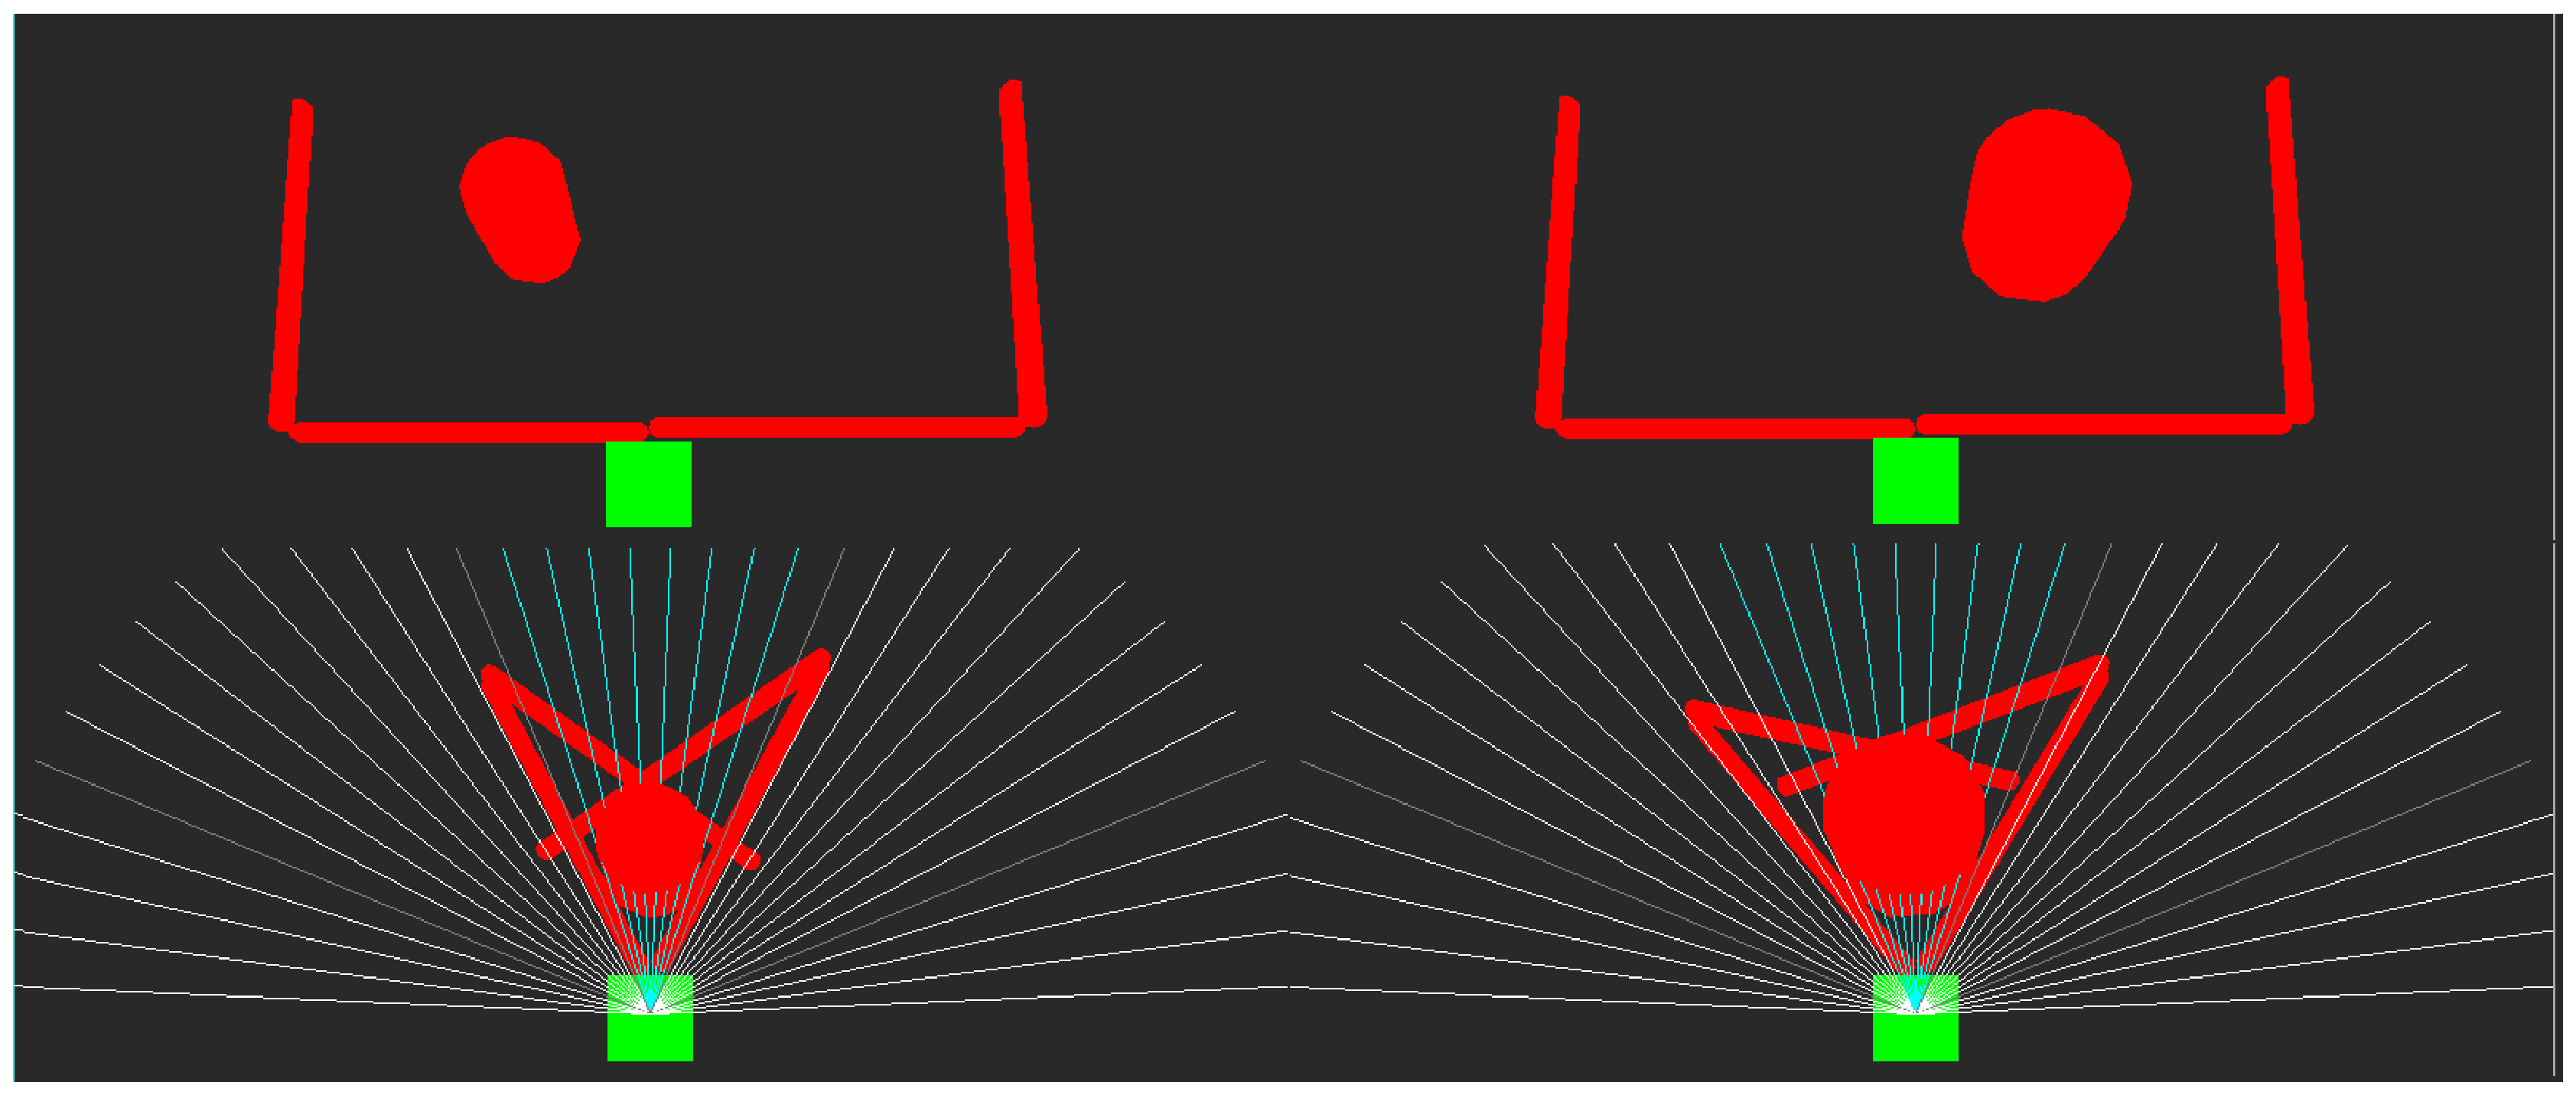
\epsfig{file=robot.eps, scale=0.15}
  \caption{Each of the four frames show the robot under different environments. The top frames depict the start of simulations with a small object and a large object respectively. The bottom frames exhibit the rays the robot uses to see objects after the robot has gripped the objects during its simulation, with the slightly darker ray depicting the center of each eye.}
  \vspace{-0.3cm} 
  \label {fig:robot}
\end{figure}

\begin{eqnarray}
  d_r &=& \sqrt{(x_{r,o} - x_{r,c})^2 + (y_{r,o} - y_{r,c})^2 + (z_{r,o} - z_{r,c})^2} \nonumber \\
  v &=& \frac{1}{N} \sum_{r=1}^{N} \begin{cases} 2 \frac{d_r}{R} - 1 & \mbox{if ray } r \mbox{ collides} \\ 1 & \mbox{otherwise} \end{cases}
\end {eqnarray}

\newpage
\subsection {Controller}

The robot's controller is a synchronous, deterministic, and real-valued neural network. Figure \ref{fig:neuralnet} reports its architecture, where each layer is fully connected to the succeeding layer. The middle (hidden) layer is also fully recurrent, obtaining inputs from all five input and five hidden neurons. The output layer's five neurons feed directly from the hidden layer. Four of the five input neurons were designated as sensor inputs. The fifth input neuron was a bias neuron permanently set to the maximum neuron value of one. Four of the five output neurons were used to control the joint motors. The final output neuron is the guess neuron, which was used for object categorization but did not influence the motion of the robot. At each time step the input neurons were encoded with the current sensor values. Each hidden neuron was then updated using:

\begin {eqnarray}
  h_i^{(t + 1)} &=& \text{erf} \left( \sum_{j=1}^{5}  n_j^{(t + 1)} w_{j,i}  + \sum_{j=1}^{5}  h_j^{(t)} w_{j,i} \right)
\end {eqnarray}

where $n_j$ and $h_j$ are the $j$th input and hidden neurons, respectively,
$w_{j,i}$ is the synaptic weight connecting neuron $j$ to neuron $i$, and
this weighted sum is normalized to a value in $[-1,+1]$ using the Gauss error function.
Synaptic weights were restricted to the range $[-1,+1]$.

The output neurons were updated using:
\begin {eqnarray}
  o_i^{(t + 1)} &=& \text{erf} \left( \sum_{j=1}^{5}  h_j^{(t + 1)} w_{j,i}  \right)
\end {eqnarray}

After the network was updated, the values of the four motor neurons were scaled to values in $[-90^o,+90^o]$ and then translated into torques by the motors, proportional
to how far the current angle was from the desired angle.

During the evolutionary runs in which the robot is weaned off proprioception and on
to vision, some mixture of proprioception and vision is supplied to the sensor
neurons, rather than feeding increasingly less proprioception to four sensor neurons
and increasingly more vision to an additional four sensor neurons.
In this way evolution does not need to learn to ignore or value sets of weights over the evolutionary run. 

\begin{figure}%[!t]
  \centering
   \begin{tikzpicture}[shorten >=1pt,->,draw=black!50, node distance=2.0cm]
    \tikzstyle{every pin edge}=[<-,shorten <=1pt]
    \tikzstyle{neuron}=[circle,fill=black!25,minimum size=15pt,inner sep=0pt]
    \tikzstyle{input neuron}=[neuron, fill=green!50];
    \tikzstyle{output neuron}=[neuron, fill=red!50];
    \tikzstyle{hidden neuron}=[neuron, fill=blue!50];
    \tikzstyle{annot} = [text width=4em, text centered]

    % Draw the input layer nodes
    \path[yshift=0.5cm] node[input neuron, pin=left:Sensor 1] (I-1) at (0,-1) {};
    \path[yshift=0.5cm] node[input neuron, pin=left:Sensor 2] (I-2) at (0,-2) {};
    \path[yshift=0.5cm] node[input neuron, pin=left:Sensor 3] (I-3) at (0,-3) {};
    \path[yshift=0.5cm] node[input neuron, pin=left:Sensor 4] (I-4) at (0,-4) {};
    \path[yshift=0.5cm] node[input neuron, pin=left:Bias] (I-5) at (0,-5) {};

    % Draw the hidden layer nodes
    \foreach \name / \y in {1,...,5}
      \path[yshift=0.5cm] node[hidden neuron] (H-\name) at (2.0cm,-\y cm) {};

    % Draw the output layer node
    \path[yshift=0.5cm] node[output neuron,pin={[pin edge={->}]right:Motor 1}, right of=H-1] (O-1) {};
    \path[yshift=0.5cm] node[output neuron,pin={[pin edge={->}]right:Motor 2}, right of=H-2] (O-2) {};
    \path[yshift=0.5cm] node[output neuron,pin={[pin edge={->}]right:Motor 3}, right of=H-3] (O-3) {};
    \path[yshift=0.5cm] node[output neuron,pin={[pin edge={->}]right:Motor 4}, right of=H-4] (O-4) {};
    \path[yshift=0.5cm] node[output neuron,pin={[pin edge={->}]right:Guess}, right of=H-5] (O-5) {};

    % Connect every node in the input layer with every node in the
    % hidden layer.
    \foreach \source in {1,...,5}
      \foreach \dest in {1,...,5}
         \path (I-\source) edge (H-\dest);
    
    %\draw (H-1) to[out=-20,in=-70] (H-3);
    \path [loop below] (H-1) edge (H-1);
    \path [bend right] (H-1) edge (H-2);
    \path [bend right] (H-1) edge (H-3);
    \path [bend right] (H-1) edge (H-4);
    \path [bend right] (H-1) edge (H-5);
    
    \path [bend right] (H-2) edge (H-1);
    \path [loop below] (H-2) edge (H-2);
    \path [bend right] (H-2) edge (H-3);
    \path [bend right] (H-2) edge (H-4);
    \path [bend right] (H-2) edge (H-5);

    \path [bend right] (H-3) edge (H-1);
    \path [bend right] (H-3) edge (H-2);
    \path [loop below] (H-3) edge (H-3);
    \path [bend right] (H-3) edge (H-4);
    \path [bend right] (H-3) edge (H-5);

    \path [bend right] (H-4) edge (H-1);
    \path [bend right] (H-4) edge (H-2);
    \path [bend right] (H-4) edge (H-3);
    \path [loop below] (H-4) edge (H-4);
    \path [bend right] (H-4) edge (H-5);

    \path [bend right] (H-5) edge (H-1);
    \path [bend right] (H-5) edge (H-2);
    \path [bend right] (H-5) edge (H-3);
    \path [bend right] (H-5) edge (H-4);
    \path [loop below] (H-5) edge (H-5);

    % Connect every node in the hidden layer with the output layer
    \foreach \source in {1,...,5}
        \foreach \dest in {1,...,5}
          \path (H-\source) edge (O-\dest);

    % Annotate the layers
    \node[annot,above of=H-1, node distance=0.5cm] (hl) {Hidden};
    \node[annot,left of=hl] {Input};
    \node[annot,right of=hl] {Output};
   \end{tikzpicture}
   \vspace{-0.3cm} 
   \caption{Neural Network of Controller}
   \vspace{-0.3cm} 
   \label{fig:neuralnet}    
\end{figure}
  
\subsection {Evolutionary Algorithm}

The Covariance Matrix Adaptation Evolution Strategy \cite{cmaes} (CMA-ES) was chosen as the real-valued optimization method. In all evolutionary trials,
only the synaptic weights in the robot's controller were evolved. All aspects of the robot's cognitive architecture and morphology remained fixed. CMA-ES evolved 75 synaptic weights, each constrained to $[-1, 1]$. The initial synapses vector was initialized with uniformly random weights in the bounded range. CMA-ES specific parameters included initializing each run with a $\sigma$ of 0.25 and a default of 16 fitness evaluations per generation. Each evaluation was composed of multiple simulations in which the robot was confronted with different objects placed at different positions. All other unmentioned parameters were kept at the default settings. Since we utilized CMA-ES as a function minimizer, our experiment attempted to minimize the error of the robot's guess as to which class the object currently in front of it belonged to. We shall use the term evolutionary run to refer to the process of evolving (training) our controllers for a given set of environments and sensor modality. 

\subsection {Environments}

The environment of the robots differ primarily through the position and size of the cylinder presented in each simulation. Each robot's controller for a given sensor modality was simulated a specific number of times, which we define as an evaluation. During training the objects were placed as described below and shown in Figure \ref{fig:positions} for each 6-simulation evaluation. The horizontal and vertical environments were chosen because they constrained the training data to one dimension. The alternating environment was chosen because it did not place both a large and a small cylinder at the same positions. Additionally, we also investigated how controllers evolved when exposed to fewer (4) and more (8) simulations. The evaluation types include:

\begin{description}
\item[Horizontal (H4, H6, H8)] The objects were placed across the X axis such that both sizes were tried at each unique position.
\item[Vertical (V4, V6, V8)] The objects were placed across the Z axis such that both sizes were tried at each unique position.
\item[Alternating (A4, A6, A8)] The objects were placed in a two-object deep rectangle, alternating large and small objects, each object with their own unique position.
\item[Testing] The objects were placed on a Cartesian plane over 78 positions for a total of 156 simulations. 
\end{description}

\begin{figure*}[!t]
  \centering
  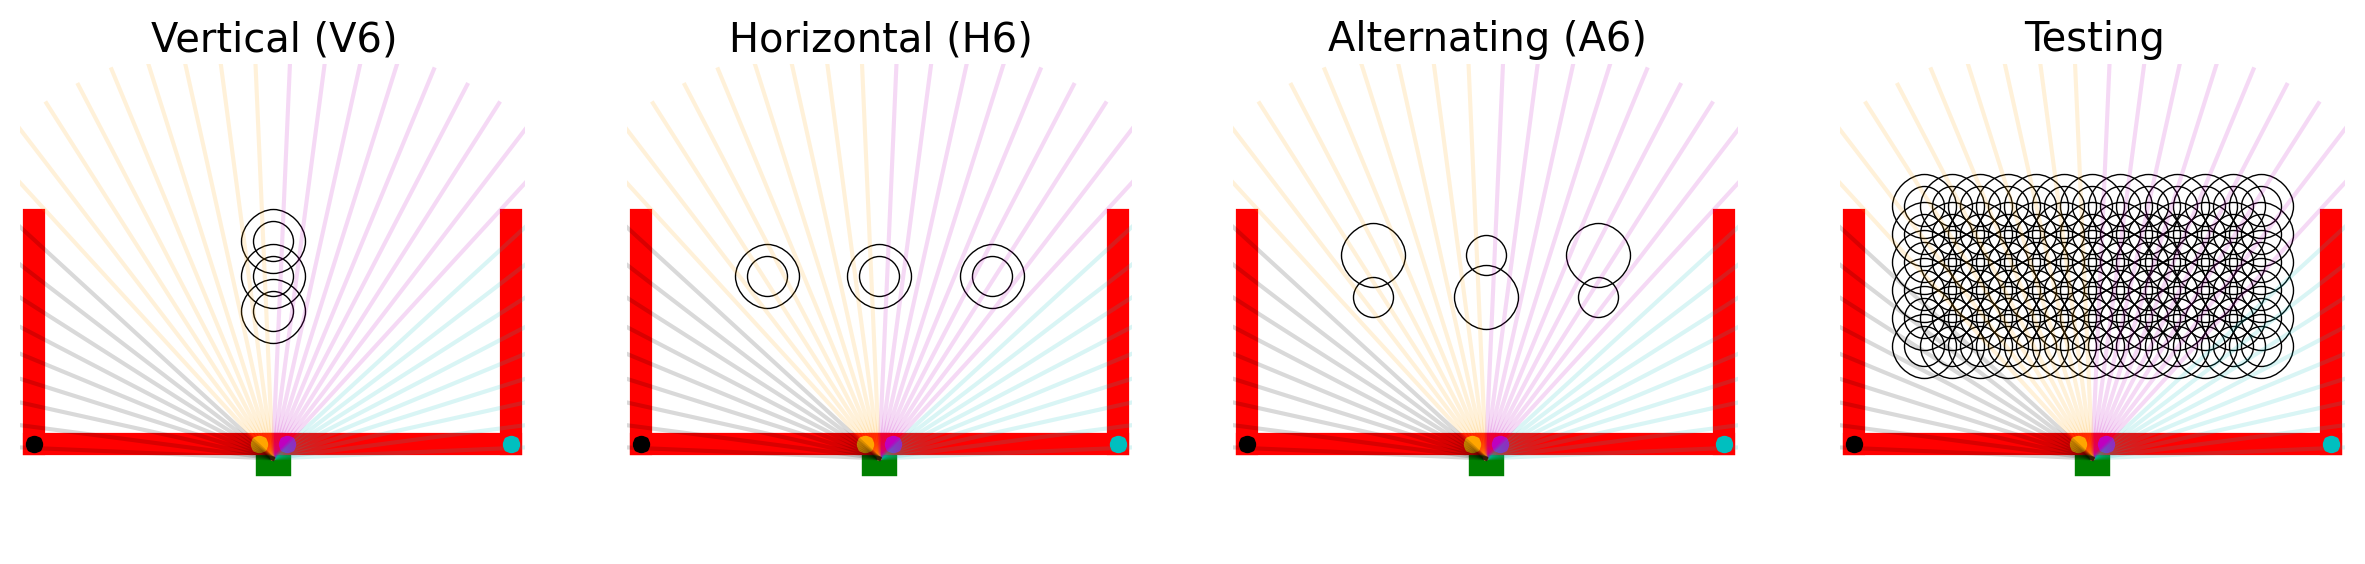
\epsfig{file=positions.png, scale=0.6}
  \vspace{-1cm} 
  \caption{ \label{fig:positions} This figure depicts the initial positions for the cylinders under various environments. Additionally, the thick red lines indicate the initial position of the robot's limbs. The filled circles represent the locations of the joints. The circle and ray colors correspond to the ordered pairs of sensors combined during the ontological scaffolding: the teal outer joint on the right arm corresponds to the rightmost eye's rays.}
  \vspace{-0.3cm} 
\end{figure*}

\subsection {Sensor Modalities and Scaffolding}

\subsubsection {Proprioception (P)}

Robots evaluated under this sensor modality only utilized their proprioceptive sensors (joint angles) as inputs to their controller for the entirety of training and testing. 

\subsubsection {Vision (V)}

Robots evaluated under this sensor modality only utilized their vision sensors (four eyes composed of distal rays) as inputs to their controller for the entirety of training and testing. 

\subsubsection {Scaffolding}

Although scaffolding is a common method employed in robotics \cite{dorigo1994robot, perkins1996robot, saksida1997shaping, bongard2011morphological, bongard2011morphologicalb},
we employed it here in a novel way. During the evolutionary process, the robot is forced to rely progressively less on proprioception and progressively more on vision to perform categorization. 
Three different types of scaffolds were attempted and reported here. For each scaffolding type, a single parameter linearly descends from one to zero over the course of an evolutionary run and dictates how much proprioceptive input the robot has access to (blue line in Figure \ref{fig:scaffolding_contribution}).
A second parameter climbs from zero to one over the course of 
an evolutionary run and dictates how much visual input the robot has access to (green line in Figure \ref{fig:scaffolding_contribution}). During testing, the controllers evolved using scaffolding were tested identically to the controllers evolved using the Vision (V) sensor modality. 

During scaffolded evolutionary runs the robot could rely only on proprioception during the initial 30\% of training. The next 60\% of training time caused a constant linear decrease in the scaffold.  During the final 10\% of training, the robot could only rely on vision.
Each robot evaluation was provided with a fraction that was zero during the first 10\% of training, some value in $[0,1]$ during the next 60\% of training, and one for the last 10\% of training.
This value was used to tune the three scaffolding schedules described next.

\begin{figure}[!t]
  \centering
  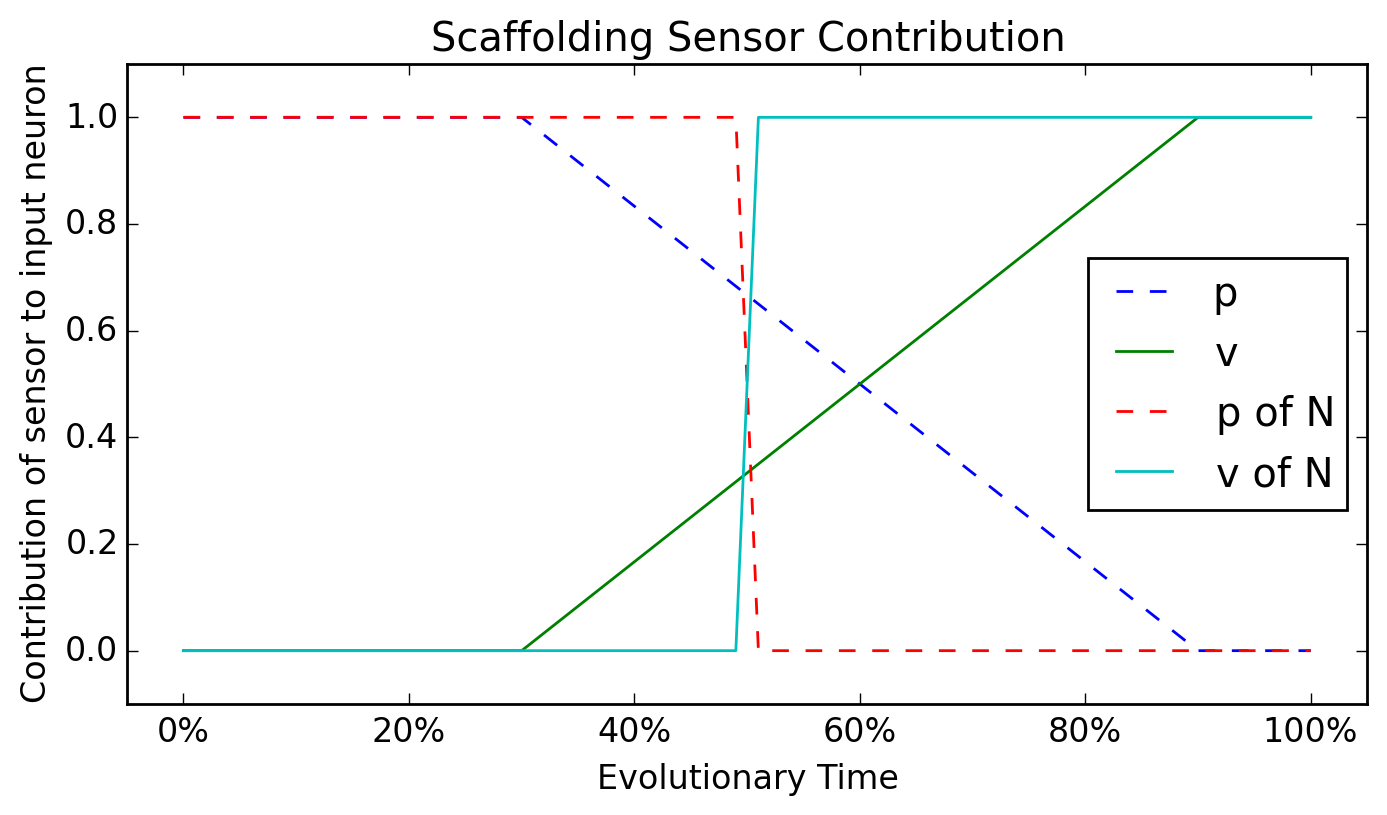
\epsfig{file=scaffolding_contribution.png, scale=0.45}
  \caption{The relative contribution of proprioception (P) and vision (V) to a robot's input over the course of an evolutionary run that is scaffolded. This parameter is then used in each simulation as seen in Figure \ref{fig:scaffolding}.}
  \vspace{-0.3cm} 
  \label{fig:scaffolding_contribution}
\end{figure}
\begin{figure}[!t]
  \centering
  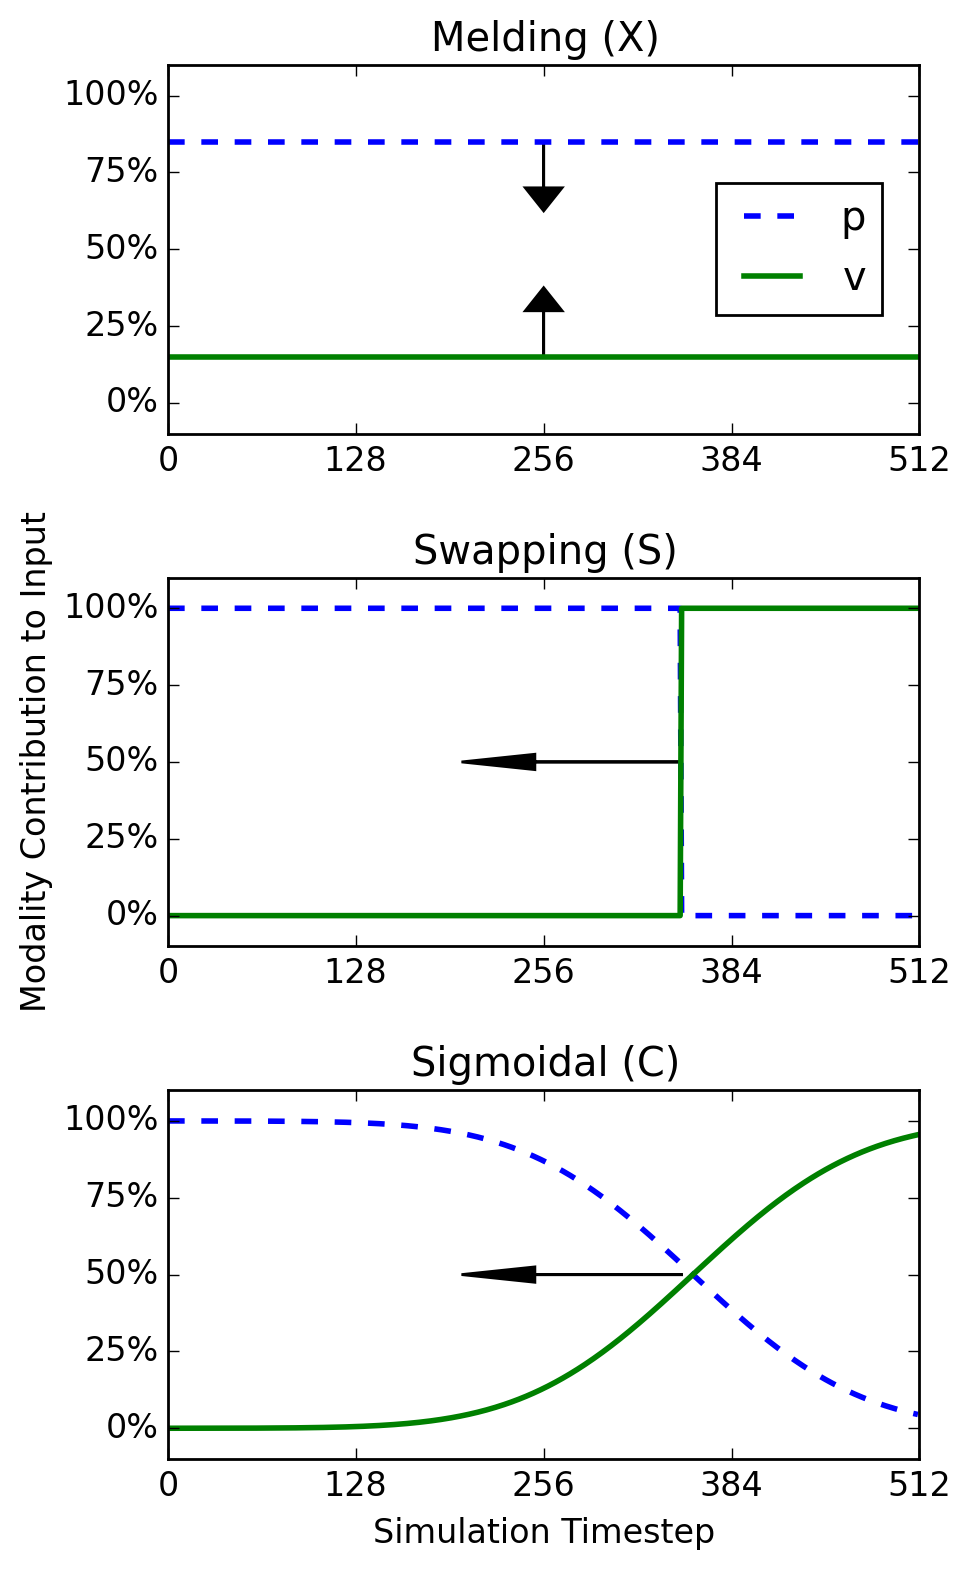
\epsfig{file=scaffolding.png, scale=0.5}
  \vspace{-0.3cm} 
  \caption{Changes in contribution of proprioception (P) and vision (V) during the evaluation of a single controller. The lines represent ontological scaffolding, or the scaffolding that occurs over one simulation of the robot. The arrows represent how the relative contribution of proprioception and vision change as the evolutionary run proceeds. The movement in the direction of the arrows, as described in Figure \ref{fig:scaffolding_contribution}, represents evolutionary scaffolding.}
  \vspace{-0.5cm} 
  \label{fig:scaffolding}
\end{figure}


\begin {description}

\item[Melding (X)] During the evaluation of an individual robot, the values arriving at the sensor neurons were an admixture of the four proprioceptive and the four visual
sensors (Fig. \ref{fig:scaffolding}a). The proportions of both sensor modalities gradually changed over evolutionary time: robots in the first generation obtained 100\% proprioceptive input and 0\% visual input, robots halfway through an evolutionary run received roughly 50\% proprioceptive input and 50\% visual input, and robots in the final generation received 100\% visual input.
\item[Swapping (S)] Partway through the evaluation of a single robot, its input would switch from proprioception to vision (Fig. \ref{fig:scaffolding}b). The point at which this swap would occur
changed over evolutionary time: robots in the first generation received only proprioceptive input, robots halfway through an evolutionary run received proprioceptive
input for the first 256 time steps and visual input for the last 256 time steps, and robots in the last generation received only visual input.
\item [Sigmoidal (C)] A sigmoidal smoothing function was used to determine the amount of contribution of vision and proprioception to the input layer during any single
  time step of the evaluation (Fig. \ref{fig:scaffolding}c). The shape of this sigmoid was altered over the course of an evolutionary run such that the contribution of proprioception dropped more precipitously---and the amount of visual input increased more precipitously---later during the evolutionary run. Essentially, this scaffold is a combination of the other two scaffolds.
\item [None (N)] For the first half of evolutionary time the robot's controller solely received input from its proprioceptive sensors. For the second half of evolutionary time the robot's controller solely received input from its vision sensors. 
\end {description}

  In the case of the sigmoidal smoothing function the contribution of vision to the value of the input neurons is shown in equation 4. The term $g$ represents the current generation in the evolutionary run out of $G$ generations. The term $t$ represents the time step in the simulation out of $T$ time steps. 
  \begin {eqnarray}
  c_v &=& \frac{ \erf \left[ 4 \left( \frac{g}{G} + 2 \frac{t}{T} - 1 \right) - 2 \right] + 1}{2}
\end {eqnarray}

\subsection {Fitness}

Each simulation lasted 512 time steps in the Bullet Physics Engine\cite{bullet}. The final 10\% of values of the controller's guess neuron were recorded and used to compute the controller's fitness. The guess neuron's values were compared against the cylinder's class label (-0.5 for small and 0.5 for large) to obtain a difference. This difference is averaged over the time steps to become our error:

\begin {eqnarray}
  e &=& \frac{1}{C} \sum_{c=1}^{C} \frac{1}{T} \sum_{t=0.9T}^{T} \left| g_{c,t} - r_{c} \right|
\end {eqnarray}

where $C$ represents the number of cylinders placed and $T$ represents the total number of time steps for an evaluation. 
$g_{c,t}$ denotes the value of the guess neuron when the robot is simulated under environment $c$ and
$r_c$ denotes the relative radius of the object in environment $c$. ($r=-0.5$ for the small object and $r=0.5$ for the large objects.)
In this way an error of zero indicates perfect and stable categorization over the last 5\% of the robot's evaluation period.
Importantly, the category values were not set to the extrema of the neuron's output range (-1 and +1) because this made the robot's
task too easy: instead, it had to hold each guess neuron  steady at the correct value for a protracted period of time.

The robot morphology and task were formulated such that there were at least four types of movement that could be used to manipulate objects. The robot could choose to not move objects by extending its joints outward. The robot could open one of its arms while closing the other to slide objects which come into contact with the closing arm away from it. The robot could close its inner joints while keeping its outer joints relatively open, leading to the object becoming trapped in a diamond-like arm pattern. Finally, the robot could fully close both arms, leading to the object becoming trapped in a triangle formed by the arms. (Figure \ref{fig:robot}) We found that the controller rarely changed its motion strategy partway through a simulation. 

\subsection {Tests}

After evolution, we assessed how robustly a robot could categorize when simulated in novel environments.
To do so, we extracted the controller with the lowest training error obtained during the final 10\% of the generations from each evolutionary run. This robot was denoted as that run's representative. 
The representative controllers were then presented with the Testing environment as shown in Fig. \ref{fig:positions}.
In these test evaluations the robots were only allowed to use the visual sensors for categorization. The only exception were those runs in which only proprioception was allowed during training; these robots were allowed to use only proprioception during testing.
As during training, testing error was calculated using Equation (5), but averaged over 156 simulations instead of four, six, or eight simulations.

In the next section we investigate the intra- and inter-category distances
between objects caused by the robot's movement. The following equations describe these values. In each case $I$ and $J$ represent the number of large and small objects, respectively. 

\begin {eqnarray}
  D_{\text{intra}} &=& \frac{2 \sum_{i=1}^{I} \sum_{j=i + 1}^{I} \sqrt{(x_i - x_j)^2 + (z_i - z_j)^2} }{I (I - 1)} \\
  &+& \frac{2 \sum_{i=1}^{J} \sum_{j=i + 1}^{J} \sqrt{(x_i - x_j)^2 + (z_i - z_j)^2} }{J (J - 1)} \nonumber \\
  D_{\text{inter}} &=& \frac{1}{I J} \sum_{i=1}^{I} \sum_{j=1}^{J} \sqrt{(x_i - x_j)^2 + (z_i - z_j)^2} 
\end {eqnarray}

\section {Results}
\label{sectResults}

In this section we report on a total of $3 \times 3 \times 6 \times 50 = 2250$ evolutionary runs. We evolved the robot's controllers against every environment: the combination of object position (horizontal, vertical, and alternating) and simulation count (4, 6, 8). Robots had six modalities: just proprioceptive input (P), just visual input (V), or evolved against one of the four scaffolding strategies (N, S, X, C). For each of the 54 combinations of object positioning, simulation count, and scaffolding strategy, we performed 50
evolutionary runs. For robots trained against four, six, and eight objects, they were evolved for 40,000, 60,000, and 80,000 robot simulations, respectively. This provided every evolutionary run with the same number of evaluations. 

The average testing errors for the representative controllers is reported in Table \ref{table:summary}. A robot whose strategy would be to randomly guess the size of its cylinders would have a test error of 0.5. When we refer to robots as memorizing we mean that their test error is high; these robots have overfitted the training examples and therefore cannot perform well on the generalized test set.


In most cases, the robots trained with vision (column 'V' in Table 1)
memorized more than robots trained using one of the scaffolds (columns
'N' through 'C' in Table 1). However, robots trained with proprioception
and then tested using proprioception also memorized on occasion: these
robots obtained similarly high testing error as the robots trained and
tested with vision in environments H6 and A4.
This result implies that although the task may seem sufficiently simple
that categorization using proprioception always results in robust
categorization in unseen environments, there are movement strategies
that evolve for which this is not the case.
In this case, the P solutions evolved behaviors that would swing the arms asymmetrically, utilizing feedback from the objects' positions to complete the task of deciding their size. 

\setlength{\tabcolsep}{4pt}
\begin {table} [!t]
  \begin {tabular}{|c|l|l|l|l|l|l|} \hline
  & P          & V    & N       & X       & S       & C       \\ \hline
  A8 & 0.16**  & 0.24 & 0.23    & 0.21    & 0.22    & 0.19*   \\ \hline
  H8 & 0.14*** & 0.23 & 0.21    & 0.21    & 0.24    & 0.21    \\ \hline
  V8 & 0.16*** & 0.27 & 0.25    & 0.25    & 0.32    & 0.27    \\ \hline \hline
  A6 & 0.21*** & 0.31 & 0.27    & 0.22*** & 0.27    & 0.25**  \\ \hline
  H6 & 0.20    & 0.22 & 0.25    & 0.22    & 0.26*   & 0.21    \\ \hline
  V6 & 0.23*** & 0.41 & 0.35**  & 0.30*** & 0.34*** & 0.35*** \\ \hline \hline
  A4 & 0.36    & 0.35 & 0.34    & 0.37    & 0.36    & 0.39    \\ \hline
  H4 & 0.20*** & 0.36 & 0.26*** & 0.26*** & 0.28*** & 0.24*** \\ \hline
  V4 & 0.20*** & 0.41 & 0.34*   & 0.35*   & 0.34**  & 0.36*   \\ \hline
  \end {tabular}
  \caption{Test errors for 50 runs over the different object counts. positions, and sensor modalities. The asterisks designate $p$ values below 0.05, 0.01, and 0.001 for one through three asterisks respectively. $p$ values were calculated by applying a t-test to the average test errors of vision when compared to other those of the other sensor modalities for each of the environments.}
  \vspace{-0.3cm} 
\label {table:summary}
\end {table}

\section{Discussion}
\label{sectDiscussion}

It was found that many scaffolded robots evolved to rely on proprioception early during an evolutionary run. These ACP-evolved behaviors contributed to contributed to the evolution of subsequent controllers that
exhibited robust visual categorization in novel environments. This is indicated by the significantly lower testing error obtained by many of the scaffolding schedules (X, S, and C) compared to the runs in which only vision was available (V). The behavior exhibited by one of these robustly-categorizing robots is illustrated in Figure \ref{fig:robot}. As can be seen, this robot's evolved behavior of closing its arms together has the effect of moving objects at different positions to the same position directly in front of the robot. This has the result of reducing differences in irrelevant properties of the
object; here, such an irrelevant difference is the different positions of the objects.

In contrast, a robot that does not move will generate no difference in sensor signatures during different object placements if it relies on proprioception for categorization, and very
different sensor signatures if it relies on vision. Neither bode well for robust categorization in unseen environments. In the former case, the robot will not be able to successfully
categorize even under training environments. In the latter case, there is a danger that the robot will memorize the training environments and fail to generalize to any unseen environments. This highlights the importance of motion for active categorical perception and that proprioception is more likely to lead to active behaviors: a blind robot must move and contact objects in order to categorize them.

\subsection {Scaffolding success through motion}

For the experiment set involving vertical arrangement of six object positions (V6), we obtained some of our most successful results. Since the training set consisted of closely positioned objects, vision-evolved controllers had a natural tendency to memorize with little movement. As shown in Figure \ref{fig:pv_V6_60} both the proprioception and all of the scaffolded runs resulted in significantly more motion during testing. This indicates that when vision favors passive behaviors that do not involve object manipulation, then scaffolding can be a good way to
bias search toward movement-based categorization. This movement-bias is retained while the robot transitions to vision, and results in increased robustness of the eventual visual classifier. 

One of the primary indicators for whether a controller would generalize was the extent to which it manipulated the object. As shown in Figure \ref{fig:pv_V6_60}, the motion induced by the vision-based controllers is significantly lower than any observed in the scaffolded runs. Memorization combined with the lack of motion is the reason that the visual classifier was only able to successfully categorize objects inside the range of its training positions. 

The scaffolding process can therefore lead to robust visual classifiers. The efficacy of scaffolding indeed increased as the training set grew increasingly sparse (eight objects
are reduced to six and then four in Table \ref{table:summary}) and accordingly the amount of computational effort available was increasingly restricted (from 80,000 robot simulations to 60,000 to 40,000).

\begin{figure} [!t]
  \centering
  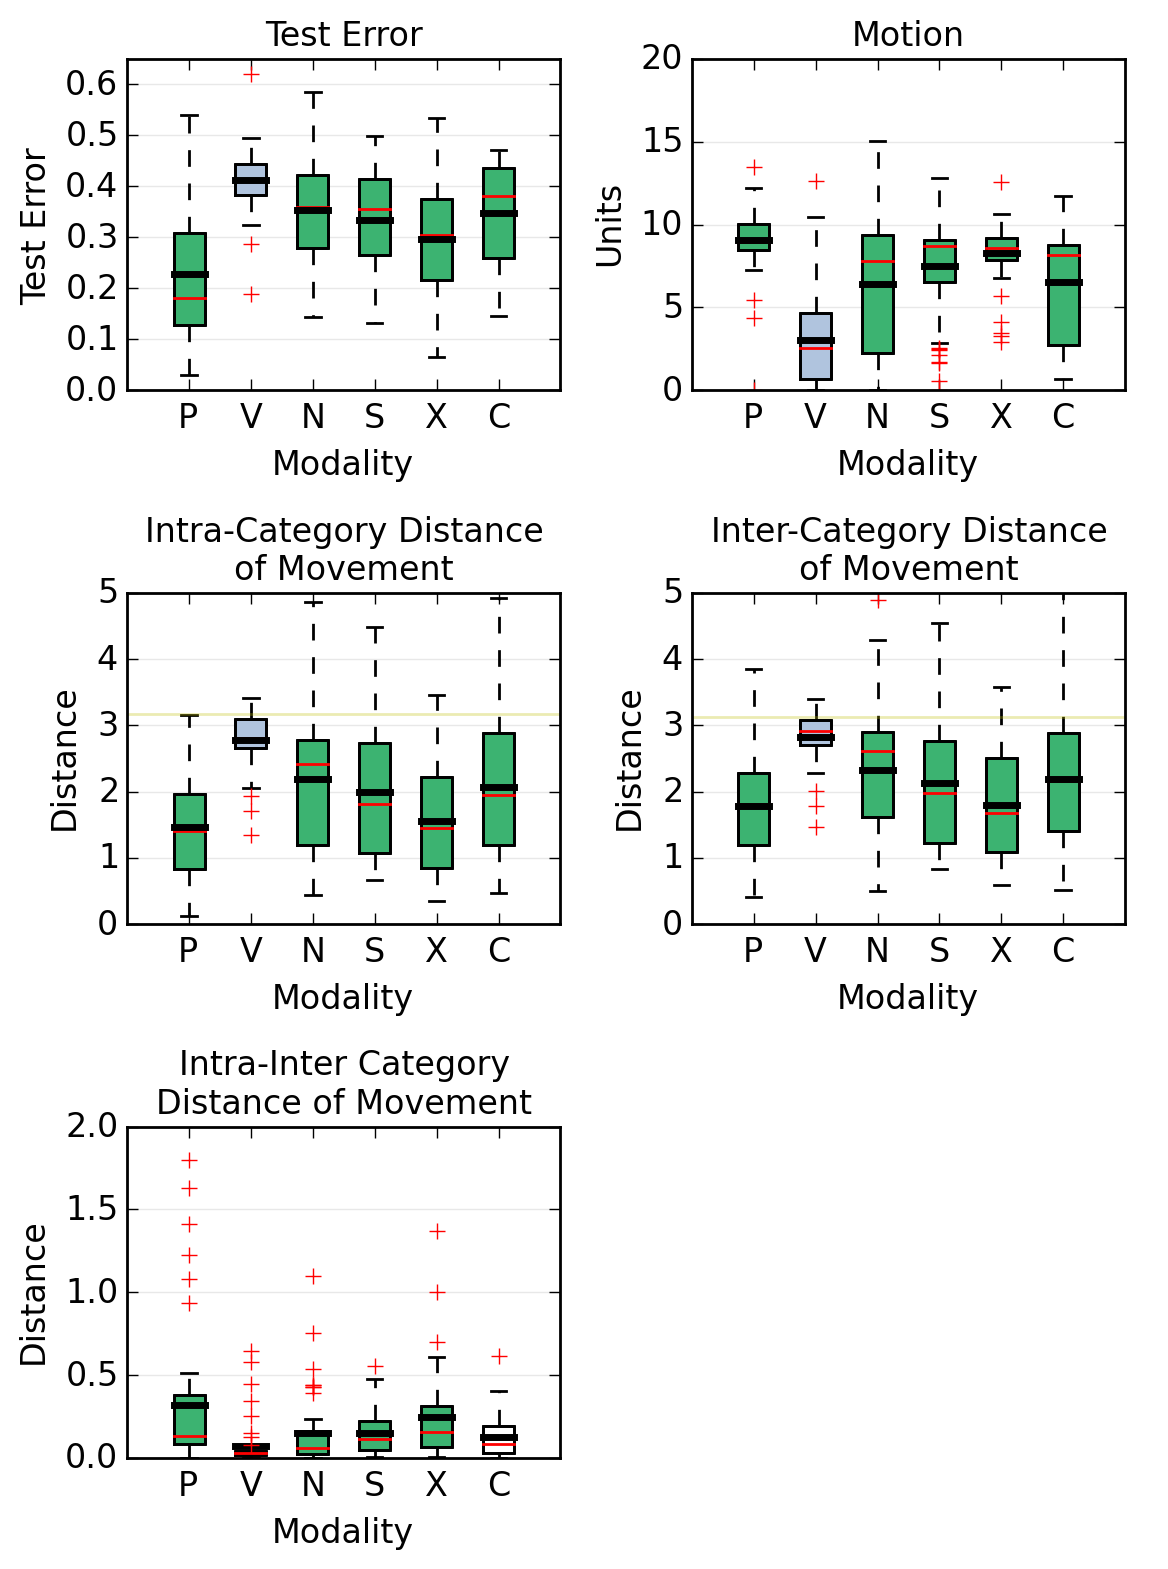
\epsfig{file=pv_gecco5_w060_vV6.png, scale=0.55}
  \vspace{-0.3cm} 
  \caption {Statistics of V6-trained controllers over 60,000 simulations per run. We define motion as the average euclidean distance between the beginning and ending positions of the objects during testing simulations. The light blue boxplot represents vision. Green boxplots for each subplot are significantly different than vision at a p level of 0.05. The horizontal red lines designate medians and the thick horizontal black lines designate the mean. In the intra and inter-category graphs the horizontal yellow lines designate what the distances would be if the test objects were not perturbed. The boxplot's whiskers represent the 25th and 75th percentiles.}
  \vspace{-0.6cm} 
  \label{fig:pv_V6_60}
\end {figure}

\begin{figure} [!t]
  \centering
  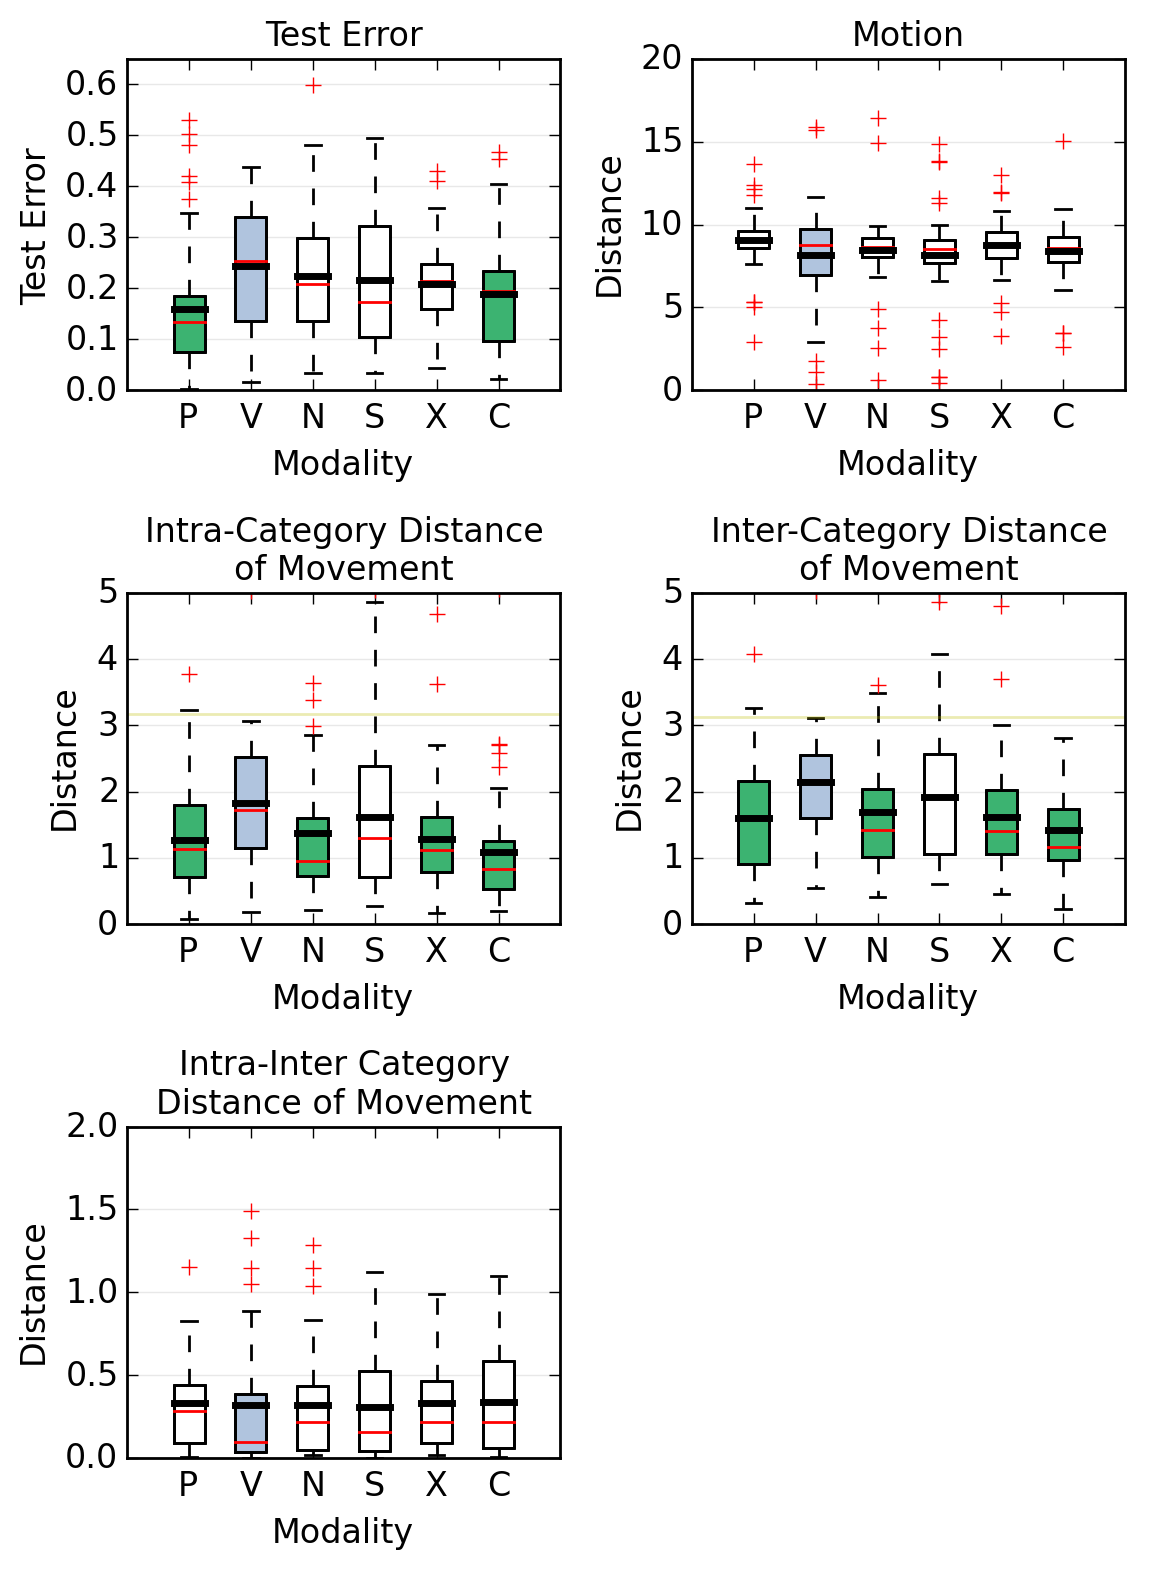
\epsfig{file=pv_gecco5_w080_vA8.png, scale=0.55}
  \vspace{-0.3cm} 
  \caption {Statistics of A8-trained controllers over 80,000 simulations per run.}
  \vspace{-0.5cm} 
  \label{fig:pv_A8_80}
\end {figure}

\subsection {Scaffolding success in other cases}

We also investigated the effect of scaffolding when the visual classifier's motion was not significantly different from robots that relied on proprioception.
This was the case for the A8 training regimen, as shown in Figure \ref{fig:pv_A8_80}. However, even in this case, the C scaffolding schedule achieved significantly lower test error than pure vision.

The reason for this is that motion is not a meaningful metric in and of itself. A robot may evolve to move its arms a great deal and push the objects away from it in ways that exaggerate the irrelevant feature of object position.

To distinguish between helpful and unhelpful motion, we can look at intra-category and inter-category distances. Intra-category distance, the average distance between the final position of an object and every other object in its category, would be low for the behavior shown in Figure \ref{fig:robot} as the objects would be pulled to about the same location. Since objects are getting pulled close regardless of size, we would expect to see inter-category distance, the average distance between an object and every other object not in its category, to also decrease a similar amount.

Because the radii of the objects are different, we do not expect inter-category distances to be lower than intra-category distances as the centers of the two object sizes would be in marginally different places (25\% of the small object's radius) when the objects are flush against the robot's chassis. For unhelpful movement, objects may be pushed away from a swinging arm or not moved at all: both intra-category and inter-category distances should thus remain high.
The results in Figure \ref{fig:pv_A8_80} show that the scaffolds that were most successful have intra-category and inter-category differences that are low, like those for proprioception.
The unsuccessful scaffold (S) characteristically evolved higher intra-category and inter-category behavior, which were more in line with the same metrics for the pure vision runs (V). 

From this, it seems likely that the best predictor of whether a particular run will produce robust visual classifiers is whether the difference between intra-category and inter-category distances is magnified by motion induced by the robot's limbs. Indeed this is what is observed in the results from the V6 training regimen (Figure \ref{fig:pv_V6_60}).

The types of movements that the scaffolds can help instigate is therefore also an important component of whether they lead to robust visual categorization, and the signature of whether motion is helpful is if it reduces the separation between intra-category and inter-category differences. 

\subsection {Scaffolding Issues}

As shown in Table \ref{table:summary}, both the vertical and horizontal environments' scaffolds lead to relatively better generalizers as we provide fewer training positions, and therefore less computational power. This highlights vision's inclination towards memorization. In the case of the alternating object positions, a different pattern emerges. In the case of A4, neither proprioception nor any of the scaffolds have significantly different means; proprioception becomes just as much a memorizer as vision. This explains the lack of success of the scaffolds; they do not have a robust categorization strategy from which to begin weaning the robot off proprioception. However, as we add computational power and complexity through A6 and A8, proprioception-based robots memorize less. Even as the environments exhibit greater variation and vision-based controllers memorize, proprioception based controllers resist memorization and are thus still able to be scaffolded. This indicates that even when problems are not constrained to a single dimension of position, there may be success through sensor scaffolding. The underlying pattern for success is whether proprioception can evolve and then pass these successful grasping behaviors to vision. The grasping behaviors that work are the ones that collapse the state space by reducing intra-category and inter-category distances. 

When comparing our four scaffolds, none of the scaffolds had a clear and universal advantage over any other. The positive aspect of this is that scaffolding strategies are a manual process that the experiment designer must consider. On the other hand, we still have little insight into the underlying intricacies of applying different scheduling scaffolds. 

\section{Conclusions and Future Work}
\label{sectConclusions}

Here we have demonstrated how, through action, a robot may be gradually
transitioned from active categorical perception to visual classification.

Direct successors to this research revolve around improving the efficacy of scaffolding. 
We believe that the current method presented in this paper can potentially benefit from further optimizations. These potential investigations include spending more time evolving proprioceptive behaviors and limiting evolution's ability to move away from ACP-evolved grasping behaviors. Another angle of approach would be provide each evolutionary run with a randomized set of initial positions to evolve with. Other future work might include evolving classifiers that utilize both touch and vision concurrently, or a system that learns to map sensors to neural inputs concurrently with the scaling of its neural weights. 

The results presented here and previously in \cite{bongard2010utility},
when taken together, suggest
a pathway for uniting the two sister disciplines of evolutionary robotics
and developmental robotics.
Work in evolutionary robotics tends to focus on how control and morphology
can be gradually shaped by evolutionary pressures to enable successful achievement
of a task \cite{bongard2013evolutionary}.
In developmental robotics, the focus is often on how an individual
robot gradually acquires greater behavioral competency as its sensory and
motor systems complexify or become less constrained \cite{lungarella2003developmental}.


If these two approaches were combined in future work, evolution may 
explore different kinds of developmental transitions from embodied to non-embodied
categorization, beyond the four manually-devised transitions we studied
here.
Evolved transitions that enable a more efficient transition from proprioception
to vision during the robot's lifetime would confer an evolutionary advantage on it, thus leading
to the evolution of increasingly efficient transitions.
This better reflects biological evolution, which evolves developmental trajectories
from infant to adult forms, rather than fixed traits.
Such a combined evolutionary and developmental approach
may discover evolved transitions that are
more efficient and effective than the manually-devised developmental transition
studied here.

Furthermore, in previous work \cite{bongard2010utility} it was shown that evolving morphology can
facilitate the acquisition of active categorical perception in robots.
Thus, evolving morphology may further empower evolution to discover
useful control, morphology and action combinations that lead to efficient
transitions from embodied to non-embodied categorization.

It may also be applicable to other aspects of cognition. For example,
it may be possible to automatically evolve embodied language understanding
\cite{fischer2008embodied} or
embodied symbol manipulation \cite{lakoff2000mathematics}, and then
automatically and gradually
transition these competencies to abstract reasoning about language or
symbols.

\bibliographystyle{abbrv}
\bibliography{gecco} 

\balancecolumns
\end{document}
